\section{FPGA design approach}
\label{sec:approach}

In this section, we present the \ac{FPGA} design denoted as \ac{ffSCITE} in terms of overall kernel structure, data representation, updates of mutation tree candidates, and parallel likelihood calculation. Although written with a specific implementation in mind, these design aspects are largely independent of the target FPGA architecture and used tool chain.

\subsection{Kernel Structure}
\label{sec:kernel_structure}

\begin{figure}[tbh]
    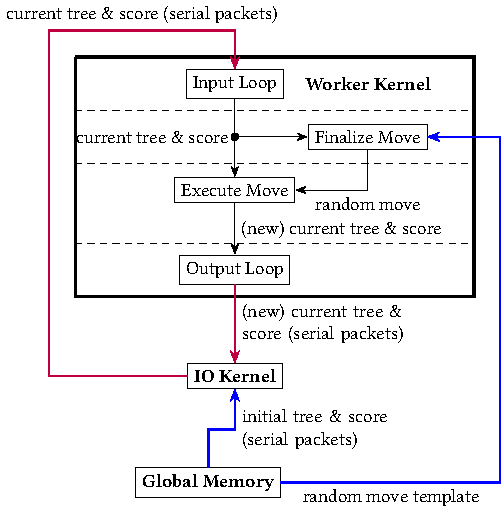
\includegraphics{figures/design.pdf}
    \Description{A block diagram with one nodes called ``Global Memory,'' ``IO Kernel,'' and ``Worker Kernel.'' The worker kernel is further subdivided into the blocks, ``Input Loop,'' ``Finalize Move,'' ``Execute Move,'' and ``Output Loop.''}
    \caption{Block diagram of the \acs{FPGA} design of \acs{ffSCITE}. The IO kernel and the worker kernel are connected via pipes, colored in violet, and the kernels access the global memory via load-store units, colored in blue. The sections separated by the dashed lines inside the worker kernel run in parallel and use/forward the values from the previous stage.}
    \label{fig:design}
\end{figure}

The general \ac{FPGA} design that realizes the \ac{MCMC} algorithm is illustrated in Fig.~\ref{fig:design} and contains a worker kernel and an IO kernel. These kernels are circularly connected using pipes realized as on-chip FIFO buffers. The IO kernel sends the current tree and its score to the worker kernel and with a design-specific latency, the worker kernel sends the result back to the IO kernel. Each transfer is done sequentially in several packets since a pipe with a sufficient bitwidth to transfer a full tree in one cycle would use excessive routing resources and would not be utilized in each cycle anyway. The worker kernel receives the current tree and its score with an input loop. Then, the kernel decides how to modify the tree. In order to save resources for a random number generator on the FPGA and since little off-chip bandwidth is used by the rest of the design, random move templates are pre-computed on the host. Before kernel invocation, they are transferred to the global memory of the accelerator card and streamed in and finalized with the knowledge of the current tree inside the worker kernel.
%We have previously computed the random numbers for this on the \ac{FPGA}, but the required pseudo-random number generator was a major bottleneck for the design. We have eliminated this bottleneck by precomputing random move templates on the host and storing them in the global memory of the accelerator card. The worker kernel only loads those templates from memory and finalizes them with the knowledge of the current tree. 
%\todo[inline]{Simplify by directly presenting the current version without the \emph{previously}.} 
Once the suggested move is decided, the ``Execute Move'' step executes the move, computes the likelihood score of the proposed tree, and decides whether the proposed tree is accepted as the new tree. As stated earlier, a proposed tree is accepted if it has a higher likelihood than the current tree or if the ratio of the proposed and the current likelihood is above a random threshold. This threshold is also fetched from global memory as part of the move template. The updated tree is fed back to the IO kernel. 
%It also internally stores the most likely tree encountered by the worker kernel and writes it back to global memory once the execution is finished.
%\tobias{Now, the updated tree could be directly fed back into input stage of the worker kernel. However, the latency for executing the move is higher than the inverse throughput of the worker kernel. Therefore, to avoid idle bubbles in the pipeline, moves on other, independent trees from other \acl{MCMC} are executed in an overlapping sequence meanwhile. To this end, the output loop sends the resulting tree back to the IO kernel, which schedules a configurable number of other, independent trees to the worker kernel before feeding the previous one back to the worker. The IO kernel also keeps track of the globally most likely candidate tree encountered by the worker kernel and writes it back to global memory once the execution is finished.}

These four parts, the input loop, the move finalization, the tree modification and scoring, and the output loop can work independently and form a meta-pipeline. The worker kernel can therefore process multiple chains at once, which is exploited by the IO kernel. It assumes a certain capacity for the worker kernel and initially feeds a corresponding number of chains into the worker kernel. Then, the previous outputs of the worker kernel are fed back into the loop, which maintains the occupation of the worker kernel despite relatively high latency of individual steps. Once the requested chain steps were executed, the output states are discarded and if more initial states are available, those are fed into the worker kernel instead of the previous output. Otherwise, the worker kernel is flushed and execution halts. The worker kernel also keeps track of the most likely candidate tree encountered so far and writes it back to global memory once the execution is finished.

\subsection{Ancestor and descendant matrices}
\label{subsec:ancestor_matrix}

\begin{figure}[tbh]
    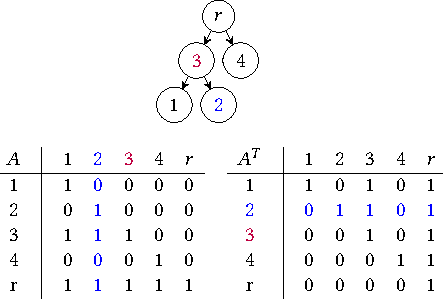
\includegraphics{figures/ancestor_matrix.pdf}

    \Description{The mutation tree from Fig.~\ref{fig:mutation_tree}, without the attached cell nodes, and the corresponding ancestor and descendant matrices below.}
    \caption{The mutation tree from Fig.~\ref{fig:mutation_tree} with the corresponding ancestor matrix $A$ and the descendant matrix $A^T$. The highlighted column \textcolor{emph}{2} in the ancestor matrix contains an entry $1$ for all nodes on the path from the root $r$ to the given node \textcolor{emph}{2}, i.e. $A[r][2] = A[3][2] = A[2][2] = 1$. Its transpose in $A^T$ is related to the mutation matrix $E$ in Fig.~\ref{fig:mutation_tree}: The first two rows are identical except for the inclusion of the root node since the cells $a$ and $b$ are attached to nodes 1 and 2, respectively. However, the fourth row of $A^T$ appears in the third and fourth row of $E$ since both $c$ and $d$ are attached to node 4, and the third row of $A^T$ does not appear in $E$ since no cell is attached to node 3.
    % Its transpose in $A^T$ is -- except for the inclusion of the root node -- identical to the mutation matrix $E$ in Fig.~\ref{fig:mutation_tree}. Note however the differences between the two matrices: column \textcolor{emph2}{3} in the ancestor matrix $A$ represents node \textcolor{emph2}{3} in the tree, which has no counterpart in the mutation matrix $E$ in Fig.~\ref{fig:mutation_tree}, because no cell is attached to it. In contrast, the mutation matrix $E$ in Fig.~\ref{fig:mutation_tree} contains two identical columns for two cells attached to node 4, whereas the ancestor matrix $A$ has one unique ancestry vector for node 4.}
    }
    \label{fig:ancestor_matrix}
\end{figure}

The main innovation in \ac{ffSCITE} is the use of an ancestor matrix as the canonical tree data structure throughout the entire design. An ancestor matrix $A$ is a matrix of binary values with a row and a column for every node in the tree. For every pair of nodes $(v,w)$, the matrix contains a 1 if and only if there is a path in the tree from $v$ to $w$, i.e. $v$ is an ancestor of $w$ (including $w$ itself). Otherwise, it contains a 0. Conversely, a descendant matrix is a matrix that has a 1 at position $(v,w)$ iff $v$ is a descendant of $w$; It is the transpose of an ancestor matrix. An example is given in Fig.~\ref{fig:ancestor_matrix}, depicting a tree on top along with the corresponding ancestor matrix $A$ and descendant matrix $A^T$ below it. This data structure makes it easy to check whether a cell $c$, attached to a node $v$, is mutated at gene $g$: $g$ is mutated if and only if $g$ is an ancestor of $v$, which is indicated by $A[g][v]=1$. We have implemented this data structure as a 1d-array of bit-vectors. One bit-vector represents one row of the ancestor matrix and each bit in it represents one matrix entry. Looking up the matrix element $A[v][w]$, therefore, involves loading the $v$-th bit-vector and isolating the $w$-th bit. On the other hand, all operations that need to be executed in parallel for an entire matrix row can be expressed as word level operations on the bit-vectors, allowing for a compact code representation that is translated into bit-parallel hardware blocks.
%The big advantage of this data structure is that operations that work independently on different bits can be unrolled and are implemented as a single, parallel, and unique logic block.

\citeauthor{tree2016} \cite{tree2016} have already used an ancestor matrix in their reference implementation to compute a tree's likelihood, but their canonical data structure is a parent vector. This is a list of node indices where the $i$-th element contains the index of the parent of node $i$. 
The parent vector allows for easy modifications of the tree structure with only a few updates to parent indices but always requires a reconstruction of the ancestor matrix for the subsequent likelihood calculation. Tree updates and translating the parent vector structure into a bit-matrix both require variable numbers of steps and are thus hard to pipeline on FPGAs. Consequently, we instead use ancestor matrices throughout the entire design and also implemented the tree modifications on them to obtain a bit-parallel and predictable \acp{FPGA} pipeline.
%This simplifies modifying the tree, but always requires a reconstruction of the ancestor matrix. It is however hard to construct ancestor matrices on \acp{FPGA} since traversing the tree requires indirection through the parent vector. This introduces an unresolvable loop-carried dependency that severely limits the throughput of the design. We have eliminated the need for the parent vector representation by finding that ancestor matrices are indeed a canonical representation of a mutation tree and developing algorithms for the tree modifications that can be efficiently implemented on \acp{FPGA}.

\subsection{Mutation tree updates}
\label{subsec:tree_updates}

\begin{figure}[tbh]
    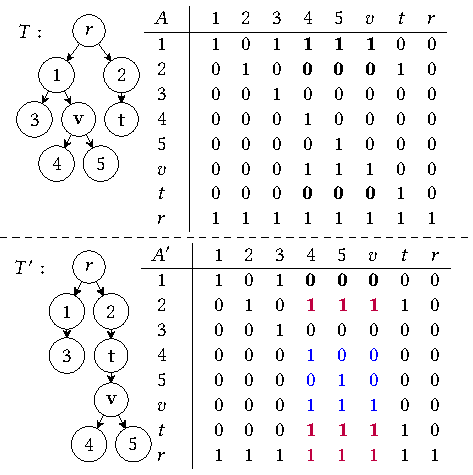
\includegraphics{figures/prune_reattach.pdf}
    \Description{A split figure with a mutation tree and its ancestor matrix on top and an altered version of the same mutation tree and its ancestor matrix below. In the altered tree, a node called ``v'' was detached from its previous parent and attached to another node called ``t;'' The ancestor matrix is changed accordingly.}
    \caption{Mutation tree and ancestor matrix representations before and after exemplary ``Prune and Reattach'' move where node $v$ is pruned from node $1$ and reattached to node $t$. Changes between $A$ and $A'$ marked in \textbf{bold}, \textcolor{emph}{colors} \textcolor{emph2}{highlight} partial rules to define $A'$.}
    \label{fig:prune_reattach}
\end{figure}

\begin{algorithm}
    \begin{algorithmic}[1]
        \STATE $A' \leftarrow 0 \in \{0,1\}^{|V| \times |V|}$
        \FORALL{$x \in V$}
            \STATE $Axt \leftarrow A[x][t]$ \COMMENT{Extract bit, 1 iff $x$ is ancestor of $t$}
            \STATE $Avx \leftarrow A[v][x]$ \COMMENT{Extract bit, 1 iff $v$ is ancestor of $x$}
            \FORALL[Parallel on complete bit-vector]{$y \in V$}  
                \IF{$A[v][y]$}\label{alg1:condition}
                    \STATE \COMMENT{Modify columns where $v$ is ancestor of $y$:}        
                    \STATE \COMMENT{\textcolor{emph2}{Connect via $t$} or \textcolor{emph}{retain subtree below $v$}}
                    \STATE $A'[x][y] \leftarrow \textcolor{emph2}{Axt} \vee \textcolor{emph}{(Avx \wedge A[x][y])}$\label{alg1:twocases}
                \ELSE
                    \STATE \COMMENT{Keep other columns}
                    \STATE $A'[x][y] \leftarrow A[x][y]$\label{alg1:keepaxy}
                \ENDIF
            \ENDFOR
        \ENDFOR
        \RETURN $A'$
    \end{algorithmic}
    \caption{Given a tree with nodes in $V$, represented as an ancestor matrix $A \in \{0,1\}^{|V| \times |V|}$, and nodes $v$ and $t$, compute the ancestor matrix $A'$ of the tree after the ``Prune and Reattach'' move with the parameters $v$ and $t$.}
    \label{alg:prune_reattach}
\end{algorithm}

In this section, we introduce the ``Prune and Reattach'' tree move as an example of the tree modification algorithms on ancestor matrices that we have developed for \ac{ffSCITE}. The other moves are similar in nature. For this move, two nodes $v$ and $t$ are sampled randomly. $v$ is sampled uniformly from all non-root nodes, but $t$ is sampled uniformly from all non-descendants of $v$ so that there is no path from $v$ to $t$ in the tree. Then, the node $v$ is moved from its current parent to node $t$. In other words, the entire subtree below $v$ is moved to a new parent. If there were a path from $v$ to $t$, the move would introduce a circle in the tree, which is why we sample $t$ from all non-descendants of $v$. Fig.~\ref{fig:prune_reattach} contains an example for this move, as well as the ancestor matrices of the tree before and after the move. In a parent vector encoding (not shown), only a single index would be changed, but in the ancestor matrix representation, multiple bits are different.

%Again, our goal now is to compute the ancestor matrix of the resulting tree from the original ancestor matrix and the move parameters. Alg.~\ref{alg:prune_reattach} builds the new ancestor matrix element by element. 
Given the inputs $A$ and the move parameters $v$ and $t$, the goal is to calculate $A'$ with simple bit-level operations. Alg.~\ref{alg:prune_reattach} presents our approach to build the new ancestor matrix element by element. 
For every pair of nodes $x$ and $y$, we find out whether there will be a path from $x$ to $y$ in the new tree. The answer to this question is the entry in the ancestor matrix for this pair. 
In the tree notation, the edge from the old parent of $v$ to $v$ is removed and a new edge from $t$ to $v$ is added. This means that the connectivity of $x$ and $y$ is only changed if the path between them would contain $v$. If there is no path from $v$ to $y$, then the potential path between $x$ and $y$ can not contain $v$. In this case, nothing changes and the entry from the old ancestor matrix is copied to the new one (Alg.~\ref{alg:prune_reattach}, lines~\ref{alg1:condition},~\ref{alg1:keepaxy}).
However, if there is a path from $v$ to $y$, then there are only two cases where a path from $x$ to $y$ can exist in the new tree: Either there is a path from $x$ to $t$, or the entire path between $x$ and $y$ is inside the subtree below $v$. If there is a path from $x$ to $t$, then we can construct a path from $x$ to $y$ via the newly introduced edge from $t$ to $v$, and if the path from $x$ to $y$ is entirely inside the subtree below $v$, then it is undisturbed by the move. The boolean expression $\textcolor{emph2}{Axt} \vee \textcolor{emph}{(Avx \wedge A[x][y])}$
%$Axt \vee (Avx \wedge A[x][y])$
(Alg.~\ref{alg:prune_reattach}, line~\ref{alg1:twocases}) covers exactly these cases, implicitly setting detached connections (in Fig.~\ref{fig:prune_reattach} the subtree below node $1$) and unrelated nodes (in Fig.~\ref{fig:prune_reattach} node $3$) to $0$.

Ancestor matrices are implemented as a list of bit vectors. The first index denotes a word in a RAM block and the second index denotes a bit in this vector. If we therefore fully unroll the inner loop over all nodes $y$, we get a single logic block that works on all bits of the vector in parallel. The hardware implementation first loads $A[v]$ to keep it in a register and then runs a single pipelined loop that loads $A[x]$, passes it through the logic, and stores the result in $A'[x]$. There are no loop-carried dependencies and the loop iteration space is fixed, unlike the ancestor matrix construction that this algorithm replaces. The other tree moves are implemented in the same way with a single pipelined loop with $|V|$ iterations and parallel logic operations per bit-vector word in the matrix.
%The other tree moves are implemented in the same way: Loading the old word from the ancestor matrix, applying combinatoric logic, and writing the results back. 
%Without these algorithms, an efficient implementation of \ac{SCITE} for \acp{FPGA} would not be possible.

\subsection{Likelihood computation}
\label{subsec:likelihood}

\begin{algorithm}[tbh]
    \begin{algorithmic}[1]
        \STATE $\mathrm{tree\_score} \leftarrow 0$
        \STATE $\mathrm{probability} \leftarrow [[\log(1-\alpha), \log(\beta)], [\log(\alpha), \log(1-\beta)]]$
        \STATE
        \FORALL[Pipelined sequentialy]{$c \in \mathrm{Cells}$}
            \STATE $\mathrm{max\_cell\_score} \leftarrow -\infty$
            \STATE
            \FORALL[Parallel, i.e. unrolled completely]{$v \in V$} \label{lst2:node_loop}
                \STATE $\mathrm{cell\_score} \leftarrow 0$
                \STATE
                \STATE \COMMENT{Cover all cases, unrolled completely}
                \FORALL{$\mathrm{prior}, \mathrm{posterior} \in \{0, 1\} \times \{0, 1\}$} \label{lst2:events_loop}
                    \STATE \COMMENT{Bit-vector load of known occurrences}
                    \STATE $\mathrm{v\_occurrences} \leftarrow \mathrm{is\_known}[c]$ 
                    \STATE
                    \STATE \COMMENT{Load and AND bit-vector of predicted cases}
                    \IF{$\mathrm{posterior} = 1$}
                        \STATE $\mathrm{v\_posterior} \leftarrow A^T[v]$
                    \ELSE
                        \STATE $\mathrm{v\_posterior} \leftarrow \neg A^T[v]$
                    \ENDIF
                    \STATE $\mathrm{v\_occurrences} \leftarrow \mathrm{v\_occurrences} \wedge \mathrm{v\_posterior}$
                    \STATE
                    \STATE \COMMENT{Load and AND bit-vector of reported cases}
                    \IF{$\mathrm{prior} = 1$}
                        \STATE $\mathrm{v\_prior} \leftarrow \mathrm{is\_mutated}[c]$
                    \ELSE
                        \STATE $\mathrm{v\_prior} \leftarrow \neg\mathrm{is\_mutated}[c]$
                    \ENDIF
                    \STATE $\mathrm{v\_occurrences} \leftarrow \mathrm{v\_occurrences} \wedge \mathrm{v\_prior}$
                    \STATE
                    \STATE \COMMENT{Compute and add score for this case}
                    \STATE $p \leftarrow \mathrm{probability}[\mathrm{posterior}][\mathrm{prior}]$
                    \STATE $\mathrm{case\_score} \leftarrow p \cdot \mathrm{popcount}(\mathrm{v\_occurrences})$ \label{lst2:popcount}
                    \STATE $\mathrm{cell\_score} \leftarrow \mathrm{cell\_score} + \mathrm{case\_score}$
                \ENDFOR
                \STATE
                \IF{$\mathrm{cell\_score} > \mathrm{max\_cell\_score}$}
                    \STATE $\mathrm{max\_cell\_score} \leftarrow \mathrm{cell\_score}$
                \ENDIF{}
            \ENDFOR
            \STATE $\mathrm{tree\_score} \leftarrow \mathrm{tree\_score} + \mathrm{max\_cell\_score}$
        \ENDFOR
        \RETURN $\mathrm{tree\_score}$
    \end{algorithmic}
    \caption{Given a tree with nodes in $V$, represented as an descendant matrix $A^T \in \{0,1\}^{|V| \times |V|}$, the mutation data matrices $\mathrm{is\_known}, \mathrm{is\_mutated} \in \{0, 1\}^{|\mathrm{Cells}| \times |V|}$, and the error probabilities $\alpha, \beta \in [0,1]$, compute the likelihood function from Subsection~\ref{subsec:likelihood}, as used in \ac{ffSCITE}.}
    \label{alg:likelihood_optimized}
\end{algorithm}

The same approach with parallel binary operations over bit-vectors and a pipelined loop over rows of the binary matrix is also applied to the likelihood calculation. 
%We have also exploited the properties of the bit-vector presentations to optimize the likelihood computation in Subsection~\ref{subsec:likelihood}: \todo{Rewrite to work without the naive implementation}
Since the original mutation matrix $D \in \{0, 1, 2\}^{|\mathrm{Cells}| \times |\mathrm{Genes}|}$ is not in a binary format, we instead encode it 
%In order to obtain simple binary operations in the central part of this computation, we encode the original mutation matrix $d \in \{0, 1, 2\}^{|\mathrm{Cells}| \times |\mathrm{Genes}|}$ 
with two binary matrices \texttt{is\_known} and \texttt{is\_mutated} $\in \{0, 1\}^{|\mathrm{Cells}| \times |V|}$. We define \texttt{is\_known}$[c][g] := (D[c][g] \neq 2)$ to encode whether the mutation status of a cell-gene combination is known, and define \texttt{is\_mutated}$[c][g] := (D[c][g] = 1)$ to encode the actual mutation status. These matrices are extended by one column such that the bit-vector format matches the one of the ancestor matrices. The \texttt{is\_known} entries for this extra column are $0$, such that it does not impact the likelihood value.
%First of all, we have transformed the input mutation matrix. Instead of using one mutation matrix $d \in \{0, 1, 2\}^{|\mathrm{Cells}| \times |\mathrm{Genes}|}$ with three possible values per cell, we use two matrices $\mathrm{is\_known}$ and $\mathrm{is\_mutated} \in \{0, 1\}^{|\mathrm{Cells}| \times |V|}$ with binary values. ``is\_known'' stores whether the mutation status of a cell-gene combination is known and ``is\_mutated'' stores the actual mutation status. We have also extended these matrices by one column so that we can use the same bit-vectors as for the ancestor matrices. This additional column, which represents the root node, is filled with unknown values so that it is not counted in the likelihood function.
%
Using these, calculating the likelihood of an attachment of a cell $c$ to a mutation tree node $v$ is possible with bit-wise logic operations. 
%With this modification, we can determine how often which event occurs by using bit-wise logic operations: Let's look at a cell $c$ which is attached to a node $v$. 
Looking at individual bits, we have a true positive mutation at gene $g$ if 
\begin{equation}
\texttt{is\_known}[c][g] \wedge \texttt{is\_mutated}[c][g] \wedge A^T[v][g]
\end{equation}
is true, which means that the cell-gene combination is reported as mutated and the underlying mutation tree model also reports the combination as mutated. 
%We have a true positive mutation at gene $g$ if $$\mathrm{is\_known}[c][g] \wedge \mathrm{is\_mutated}[c][g] \wedge A^T[v][g]$$ is true, which means that the cell-gene combination is reported as mutated and the underlying mutation tree model also reports the combination as mutated. 
Encoded as a complete bit-vector with word-level binary operations, the vector 
\begin{equation}
\label{eq:vector}
\texttt{is\_known}[c] \wedge \texttt{is\_mutated}[c] \wedge A^T[v]
\end{equation}
contains a $1$ bit for every true positive that has occurred for this cell and these occurrences can be counted with the so-called popcount function. Conversely, using the inverse $\neg\texttt{is\_mutated}[c]$ vector allows to find and count false positives, and using the inverse $\neg\mathrm{A^T[v]}$ for false respectively true negatives. The thus counted number of event occurrences is then multiplied by the respective logarithmic probability of the event and summed up to receive the log-likelihood of the entire cell attachment.
%This means that the bit-vector $$\mathrm{is\_known}[c] \wedge \mathrm{is\_mutated}[c] \wedge A^T[v]$$ contains a one for every true positive that has occurred for this cell. Conversely, the bit-vector $$\mathrm{is\_known}[c] \wedge \neg\mathrm{is\_mutated}[c] \wedge A^T[v]$$ contains a one for every false positive that has occurred for this cell, and so forth for the true and false negatives. If we count the ones in these bit-vectors with the so-called popcount function, we get the number of occurrences for every event, which we can multiply with the logarithmic probability of the event and sum up to receive the log-likelihood of the entire cell attachment.

Alg.~\ref{alg:likelihood_optimized} utilizes this way of computing the log-likelihood. The log-likelihood has the same ordering properties as the likelihood, but allows to replace exponentiation with multiplication (Alg.~\ref{alg:likelihood_optimized}, line~\ref{lst2:popcount}).
In order to find the most likely attachment of each cell to a node, the likelihood calculation of \ac{SCITE} as well as Alg.~\ref{alg:likelihood_optimized} originally contain three nested loops, one over cells, one over possible attachments (i.e. nodes in $A^T$) and one over genes per cell or node.
Following the vector-level notation of Eq.~\ref{eq:vector}, Alg.~\ref{alg:likelihood_optimized} replaces the loop over genes by bit-vectors that automatically yield parallel operations.
%In contrast to the reference outline in Alg.~??, the loop over all genes no longer shows up, because it is replaced by binary operations on bit-vectors and popcount invocations. 
On the other hand, to explicitly cover the four possible event classes with their respective \texttt{probability[posterior][prior]} values, Alg.~\ref{alg:likelihood_optimized} contains an explicit loop over all possible events (line~\ref{lst2:events_loop}). In order to generate parallel operations for these four classes, the loop is annotated with the unrolling attribute and will be specialized at compile time to the specific cases.
%Instead of summing up individual \texttt{probability[posterior][prior]} values, there is now only a single multiply-add step for each event class. On the other hand, Alg.~\ref{alg:likelihood_optimized} now contains a pair of explicit loops to iterate these four classes, which however after adding an unrolling attribute get fully evaluated at compile-time to form four separate datapaths, one for each class. 
To balance the throughput of the likelihood calculation with that of the other steps, we also mark the next loop dimension (line~\ref{lst2:node_loop}) with an unrolling attribute, which reduces the sequential steps of this function from cubic to linear, with a quadratically scaling bit-parallel datapath, which processes $4*|V|^2$ bits per clock cycle.
%replaced by bit-level AND and popcount operations and is therefore fully unrolled. The loops over the posterior and prior cases are unrolled too, which eliminates the case distinctions and the array accesses in the loop's body via constant propagation. This implementation of the log-likelihood function works exceptionally well on \acp{FPGA} due to its simplicity and we were also able to unroll one additional dimension. The resulting loop, which originally had a cubic runtime, therefore has a linear runtime and quadratic space utilization in \ac{ffSCITE}.

